\section{Công cụ Joern}

\subsection{Đặc tả đồ thị thuộc tính mã nguồn của Joern}

Đồ thị thuộc tính mã nguồn đã được nghiên cứu rộng rãi, có rất nhiều phiên bản cài đặt được xây dựng dành cho các mục đích khác nhau \cite{yamaguchi2014modeling, xiaomeng2018cpgva, kuchler2022representing, githubGitHubWimkeirgraft, githubGitHubPlumeossplume, joernJoernHunteraposs, fraunhoferaisecHomeCode, banse2021cloud, weiss2022language, keirsgieter2020graft}.
Tuy nhiên có một phiên bản mã nguồn mở được do chính tác giả của đồ thị thuộc tính mã nguồn, Fabian Yamaguchi, đích thân phát triển và duy trì có tên Joern \cite{joernJoernHunteraposs}.

Dự án CPG [6, 8] cho phép biểu diễn mã nguồn của các ngôn ngữ lập trình khác nhau dưới dạng đồ thị.
Cho đến nay, trọng tâm là Java và C/C++ nhưng hỗ trợ thử nghiệm cho Python, Go và TypeScript cũng có sẵn.
Mục tiêu của dự án là cung cấp một cách biểu diễn mã nguồn không phụ thuộc vào ngôn ngữ.
Điều này cho phép chuyên gia bảo mật xác định các lỗ hổng hoặc lỗi.
Hơn nữa, thư viện CPG bao gồm một cách để lưu trữ đồ thị trong neo4j2 và làm cho đồ thị có thể truy cập qua giao diện dòng lệnh.
Trong một số trường hợp, thư viện cũng có thể đánh giá giá trị mà một nút có thể giữ.
Tất cả những điều này cho phép chuyên gia bảo mật viết các truy vấn tùy chỉnh cho cơ sở dữ liệu đồ thị hoặc cách biểu diễn CPG trong bộ nhớ.
Thư viện CPG được thiết kế để cho phép tái sử dụng các truy vấn này giữa tất cả các ngôn ngữ lập trình được hỗ trợ.
Để đạt được mục tiêu này, thư viện CPG thực hiện một hệ thống phân cấp lớp đầy đủ, bao gồm các loại câu lệnh và biểu thức khác nhau.
CPG mã hóa thông tin như hệ thống phân cấp lớp của mã đang được phân tích, đồ thị luồng điều khiển và đồ thị cuộc gọi trong một đồ thị duy nhất.
Thiết kế hiện tại chủ yếu nhắm vào các ngôn ngữ lập trình hướng đối tượng.
Để đối phó với khả năng thiếu một số đoạn mã hoặc lỗi trong mã, thư viện có khả năng chịu lỗi với mã không đầy đủ, không biên dịch được và thậm chí ở mức độ nào đó còn không chính xác.

% Đồ thị thuộc tính mã nguồn (Code Property Graph - CPG) là một cấu trúc dữ liệu được thiết kế để khai thác các cơ sở mã nguồn lớn nhằm tìm kiếm các mẫu lập trình.
% Những mẫu này được hình thành trong một ngôn ngữ đặc thù (DSL) dựa trên Scala.
% CPG đóng vai trò như một biểu diễn chương trình trung gian duy nhất cho tất cả các ngôn ngữ được Joern và phiên bản thương mại của nó là Ocular hỗ trợ.

% Đồ thị thuộc tính là một trừu tượng chung được hỗ trợ bởi nhiều cơ sở dữ liệu đồ thị đương đại như Neo4j, OrientDB và JanusGraph.
% Trên thực tế, các phiên bản cũ của Joern đã sử dụng các cơ sở dữ liệu đồ thị mục đích chung làm nơi lưu trữ và ngôn ngữ truy vấn đồ thị Gremlin.
% Tuy nhiên, khi những hạn chế của cách tiếp cận này trở nên rõ ràng theo thời gian, chúng tôi đã thay thế cả hệ thống lưu trữ và ngôn ngữ truy vấn bằng cơ sở dữ liệu đồ thị OverflowDB của riêng mình.

Các thành phần cấu thành đồ thị thuộc tính mã nguồn bao gồm:

\begin{itemize}
  \item \textbf{Các nút và loại của chúng:} Các nút đại diện cho các thành phần của chương trình.
  Điều này bao gồm các cấu trúc ngôn ngữ cấp thấp như phương thức, biến, và cấu trúc điều khiển, cũng như các cấu trúc cấp cao hơn như điểm cuối HTTP hoặc các kết quả phân tích.
  Mỗi nút có một loại, loại này chỉ ra loại thành phần chương trình mà nút đó đại diện, ví dụ, một nút với loại METHOD đại diện cho một phương thức, trong khi một nút với loại LOCAL đại diện cho khai báo của một biến cục bộ.
  \item \textbf{Cạnh có nhãn:} Quan hệ giữa các thành phần chương trình được biểu diễn thông qua các cạnh giữa các nút tương ứng của chúng.
  Ví dụ, để biểu thị rằng một phương thức chứa một biến cục bộ, chúng ta có thể tạo một cạnh với nhãn CONTAINS từ nút của phương thức đến nút của biến cục bộ.
  Bằng cách sử dụng các cạnh có nhãn, chúng ta có thể biểu diễn nhiều loại quan hệ khác nhau trong cùng một đồ thị.
  Hơn nữa, các cạnh có hướng để biểu thị, ví dụ, rằng phương thức chứa biến cục bộ nhưng không phải ngược lại.
  Nhiều cạnh có thể tồn tại giữa cùng hai nút.
  \item \textbf{Cặp khóa-giá trị:} Các nút mang các cặp khóa-giá trị (thuộc tính), trong đó các khóa hợp lệ phụ thuộc vào loại nút.
  Ví dụ, một phương thức có ít nhất tên và chữ ký, trong khi một khai báo biến cục bộ có ít nhất tên và loại của biến được khai báo.
\end{itemize}

Tóm lại, đồ thị thuộc tính mã nguồn là các đồ thị có hướng, được gán nhãn cạnh, và chứa các thuộc tính, và chúng tôi khẳng định rằng mỗi nút mang ít nhất một thuộc tính chỉ ra loại của nó.
Điều này giúp cho việc phân tích mã nguồn trở nên dễ dàng và hiệu quả hơn, đồng thời mở ra nhiều khả năng cho việc tìm kiếm và phát hiện các mẫu lập trình trong các cơ sở mã nguồn lớn.

\begin{itemize}
  \item Đặc tả CPG của Joern được thiết kết chủ yếu cho ngôn ngữ C/C++ và Java, đưa ra các chuẩn chung như (if else, swtich case, while, for, ...) mà nhiều ngôn ngữ khác có điểm tương đồng như Python, Go, TypeScript, ... có thể tuân thủ.
  \item Tuy nhiên chuẩn chung này không thể đáp ứng được nhu cầu của tất cả các ngôn ngữ. Joern tập trung cho 2 ngôn ngữ lớn là C/C++ và Java do vậy sẽ đặc tả có sẵn (hiện có) sẽ phù hợp với các ngôn ngữ có cú pháp C-like và hướng đối tượng (OOP)
  \item Trong khi đó Rust là một ngôn ngữ lập trình mới, có cú pháp dựa trên C-Like nhưng vẫn có đôi chút sự khác biệt vì đây là ngôn ngữ hiện đại, hỗ trợ đan xen cả hướng đối tượng và hướng hàm. Đặc biệt với tính hướng hàm, Rust có nhiều cú pháp mới mà Joern chưa hỗ trợ, hay những biểu thức, mệnh đề trong C/C++ hay Java là không hợp lệ nhưng trong Rust thì hoàn toàn có thể
  \item Nhìn chung bản đặc tả CPG của Joern cung cấp 1 baseline bao phủ các tính năng phổ biến mà ngôn ngữ lập trình nào cũng có (cùng ý nghĩa nhưng có thể sử dụng cú pháp, keyword khác nhau) như $if\ else$, ... nhưng không thể đáp ứng được tất cả các ngôn ngữ lập trình hiện đại. Do vậy đối với từng ngôn ngữ riêng biệt vẫn phải bổ sung thêm các đặc tả mới cho phù hợp với từng ngôn ngữ, đặc biệt là Rust có cơ chế quản lý bộ nhớ an toàn thể hiện qua các tính năng $ownership$, $borrowing$, $lifetime$ mà Joern chưa hỗ trợ, và cả tính năng hướng hàm
\end{itemize}

\textbf{Joern Backend, Joern Frontend}

\begin{figure}[H]
  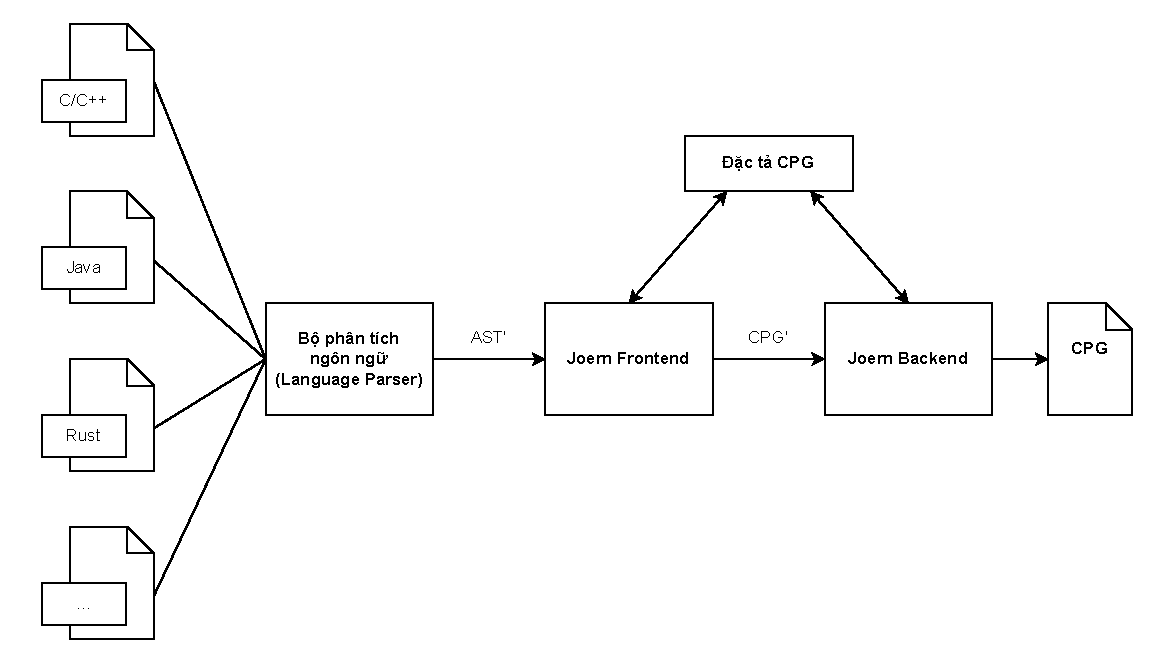
\includegraphics[width=1\columnwidth]{figures/c2/c2_frontend_backend.drawio.pdf}
  \centering
  \caption{Cách hoạt động của công cụ Joern.}
  \label{img:c2_frontend_backend}
\end{figure}

\begin{itemize}
  \item Ngoài phần đặc tả CPG dùng chung cho nhiều ngôn ngữ trên lý thuyết, Joern còn cung cấp 1 kiến trúc cài đặt thực tế có tính mở rộng cao, tương ứng với đặc tả CPG. Joern hiển tại hỗ trợ rất nhiều ngôn ngữ C/C++, Java, Python, Go, TypeScript, ... Để có thể hỗ trợ được nhiều ngôn ngữ như vậy thì Joern sử dụng 2 thành phần chính là Joern Frontend và Joern Backend, đây là 2 thành phần có tính tái sử dụng cao, không phụ thuộc vào ngôn ngữ
  \item Luồng hoạt động của kiến trúc Joern như sau. Mỗi ngôn ngữ có tập các cú pháp khác nhau, tương ứng cũng sẽ có định nghĩa về cây AST khác nhau, đây là phần người dùng muốn mở rộng Joern cho 1 ngôn ngữ mới cần phải tự đảm nhiệm. Mã nguồn của 1 ngôn ngữ sau được được công cụ Language Parser chuyển thành cây $AST*$. Cây $AST*$ ở đây không nhất thiết chỉ dừng ở đúng mức độ thông tin là 1 cây AST mà có thể bổ sung thêm thông tin khác như kiểu dữ liệu, vị trí trong mã nguồn, ... nhưng tối thiểu đảm bảo đủ thông tin là 1 cây AST tối thiểu. Ví dụ như các ngôn ngữ có sự phát triển lâu dài như C/C++ hay Java sử dụng CDT/ JDT để làm Language Parser. CDT/JDT là công cụ rất mạnh, được dùng trong các IDE nên số lượng thông tin rất đáng kể. Còn những ngôn ngữ hiện đại như Rust, Go thì các công cụ như này chưa được phát triển toàn diện nên thông tin của cây $AST*$ chưa được đầy đủ. \item Sau khi có cây $AST*$, cây này sẽ được biến đổi thành đồ thị thuộc tính mã nguồn (CPG) theo định nghĩa đặc tả CPG. Đây là công việc của Joern Frontend. Joern Frontend sẽ đọc cây $AST*$ và chuyển đổi thành đồ thị thuộc tính mã nguồn (CPG) theo đặc tả CPG. Joern Frontend đối với từng ngôn ngữ cũng là công việc cần thực hiện, do công việc thực tế cần làm là chuyển đổi cấu trúc dữ liệu của cây $AST*$ sang cấu trúc dữ liệu tương ứng của định nghĩa $CPG$. Joern Frontend đóng vai trò chuyển đổi cây $AST*$ sang cây $CPG$, $CPG$ bổ sung thông tin thành đồ thị $CPG$
  \item Sau khi được Joern Frontend xử lý, ta sẽ có được đồ thị $CPG*$ nhưng đồ thị $CPG*$ này là đồ thị không hoàn chỉnh. Để hoàn thiện được đồ thị $CPG$ thì ta cần phải sử dụng đến Joern Backend. Ở bước Joern Frontend, ta thực hiện bước chuyển đổi 1 node AST thành 1 node CPG, tạo thêm các cạnh để thể hiện các mối quan hệ giữa các node, tuy nhiên các cạnh này chưa thể hiện được đầy đủ đồ thị CPG bao gồm AST, CFG, PDG. Với cấu trúc dữ liệu CPG của Joern, ta chỉ cần định nghĩa 1 phần số cạnh, node cần thiết của đồ thị CPG, phần còn lại sẽ được Joern Backend thực hiện các thuật toán logic để có thể tự động suy diễn các mối quan hệ còn lại. Ví dụ trong cây AST có nút thể hiện vòng lặp $for$, ta chuyển thành nút $for$ của CPG kèm thêm 1 số thông tin như mệnh đề điều kiện, biến chỉ số vòng lặp (index). Joern Backend nắm được thông tin này thì có thể tự động suy diễn ra các mối quan hệ như $REACHING_DEF$ (du pair), $DOMINATOR$, $POST\ DOMINATOR$, $CONTROL\ DEPENDENCY$, $DATA\ DEPENDENCY$, $CONTROL\ FLOW$, $DATA\ FLOW$, ... từ đó tạo ra đồ thị CPG hoàn chỉnh. Chú ý CPG được cấu tạo từ 3 thành phần AST, CPG, PDG. Trong Joern thông tin của 3 thành phần này được chia thành 3 lớp, 1 đồ thị CPG được cấu tạo từ nhiều lớp trồng lên nhau, có thể sinh ra CPG chỉ có lớp AST, hoặc AST + CPG, hoặc AST + CPG + PDG. Hoàn toàn có thể mở rộng viết thêm các lớp khác nếu cần thiết, ví dụ như bổ sung 1 lớp thông tin về bảo mật, an toàn bộ nhớ, hay cụ thể trong Rust là lớp chứa thông tin $ownership$, $borrowing$, $lifetime$
  \item Sau khi toàn bộ thông tin của CPG được hoàn chỉnh dựa trên các lớp, dữ liệu CPG được xuất ra thành file binary, cấu trúc dữ liệu đồ thị. Dữ liệu này có thể được sử dụng để truy vấn thông qua các engine cơ sở dữ liệu đồ thị như neo4j, OrientDB, JanusGraph, ... hoặc có thể được sử dụng để phân tích, tìm kiếm thông qua các công cụ khác như Joern CLI, Joern Scan, Joern Slice, Joern Flow, Joern Export, Joern Vectors
\end{itemize}

\subsection{Bộ công cụ của Joern}

\begin{figure}[H]
  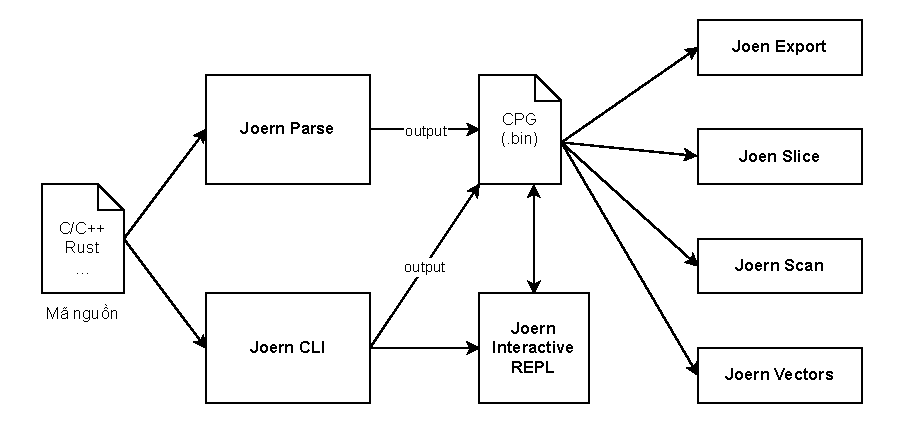
\includegraphics[width=1\columnwidth]{figures/c2/c2_joern_tools.drawio.pdf}
  \centering
  \caption{Các công cụ xung quanh Joern.}
  \label{img:c2_joern_tools}
\end{figure}

\begin{itemize}
  \item Không chỉ cung cấp kiến trúc để có thể biến đổi mã nguồn từ một ngôn ngữ sang đồ thị thuộc tính mã nguồn. Joern cần cung cấp 1 loạt các cung cấp để khai thác thông tin từ đồ thị thuộc tính mã nguồn sinh ra. Các công cụ này bao gồm: Joern Scan, Joern Slice, Joern Flow, Joern Export, Joern Vectors
  \item \textbf{JoernExport}: https://docs.joern.io/export/
  Dump intermediate graph representations (or entire graph) of code in a given export format
  Joern is used in academic research as a source for intermediate graph representations of code, particularly in machine learning and vulnerability discovery applications [e.g., 1,2,3,4,5]. To support this use-case, Joern provides both plotting capabilities in the interactive console as well as the joern-export command line utility.
  You can also export the entire graph into a neo4j csv format (along with instructions on how to import it into a running neo4j instance), graphml, graphson or graphviz dot:
  \item \textbf{JoernParse}: parse ra output ngay lập tức hoặc lưu vào cơ sở dữ liệu, không traverl
  \item \textbf{JoernSlice}: Extract various slices from the CPG.
  https://docs.joern.io/cpg-slicing/
  joern-slice is the entrypoint for Joern’s CPG slicing mechanism and specifies ways to extract useful subsets of information from the CPG. Two modes are available:
  Data-flow: This is a pretty standard backwards data-flow slicing command that starts at call arguments and slices backwards to create a graph of slices.
  Usages: This targets locals and parameters and traces what calls they make and in which calls they are used. This is useful for describing how a variable interacts in a procedure.
  \item \textbf{JoernScan}: Creates a code property graph and scans it with queries from installed bundles. QueryDB
  https://docs.joern.io/scan/
  Joern Scan ships with a default set of queries, the Joern Query Database. This set of queries is constantly updated, and contributions are highly encouraged https://github.com/joernio/joern/tree/master/querydb.
  \item \textbf{JoernVectors}: Extract vector representations of code from CPG, JoernFlow: Find flows, JoernCLI: REPL for Joern
\end{itemize}

Joern là một nền tảng mạnh mẽ dành cho việc phân tích mã nguồn, bytecode và mã nhị phân.
Công cụ này tạo ra các đồ thị thuộc tính mã nguồn (code property graphs), một cách biểu diễn đồ thị của mã giúp cho việc phân tích mã nguồn đa ngôn ngữ trở nên dễ dàng hơn.
Các đồ thị thuộc tính mã nguồn được lưu trữ trong một cơ sở dữ liệu đồ thị tùy chỉnh, cho phép khai thác mã nguồn thông qua các truy vấn tìm kiếm được xây dựng trong một ngôn ngữ truy vấn đặc thù dựa trên Scala.
Joern được phát triển với mục tiêu cung cấp một công cụ hữu ích cho việc khám phá lỗ hổng bảo mật và nghiên cứu phân tích chương trình tĩnh.

Joern hỗ trợ các nhà phát triển và nhà nghiên cứu trong việc tìm kiếm và xác định các điểm yếu tiềm ẩn trong mã nguồn, giúp nâng cao chất lượng và bảo mật của phần mềm.
Bên cạnh đó, Joern còn có khả năng phân tích mã nguồn đa ngôn ngữ, giúp các nhóm phát triển có thể làm việc với nhiều ngôn ngữ lập trình khác nhau mà không gặp trở ngại về công cụ.
Với khả năng truy vấn mạnh mẽ và linh hoạt, Joern đã trở thành một công cụ quan trọng trong việc phân tích mã nguồn và phát hiện các lỗ hổng bảo mật.
Bạn có thể tìm hiểu thêm về Joern tại địa chỉ https://joern.io/.

Joern hỗ trợ nhiều ngôn ngữ lập trình khác nhau.
Các ngôn ngữ được hỗ trợ bao gồm C/C++, Java, JavaScript, Python, x86/x64, JVM Bytecode, Kotlin, PHP, Rust, Swift, Ruby và C\#.
Điều này cho thấy Joern có khả năng phân tích mã nguồn đa ngôn ngữ, giúp các nhà phát triển và nhà nghiên cứu có thể làm việc với nhiều ngôn ngữ lập trình khác nhau mà không gặp trở ngại về công cụ.
Tuy nhiên, Joern chưa hỗ trợ cho ngôn ngữ Rust.
